\ifdefined\COMPILINGFROMMAIN
\else
    %%%%HEADER
\documentclass[twocolumn]{article}
\usepackage[a4paper, margin=1in, columnsep=20pt]{geometry}
\usepackage{amsmath, amssymb, graphicx, hyperref}
\usepackage[most,skins,breakable]{tcolorbox}
\usepackage[symbol]{footmisc}
\usetikzlibrary{calc}
\usepackage{xcolor}
\usepackage{caption}
\usepackage{algorithm}
\usepackage{algpseudocodex}
\usepackage{tikz}
\usepackage{listings}
\usetikzlibrary{arrows.meta, positioning}
\tcbuselibrary{listingsutf8}
\usepackage{microtype}
\usepackage{blindtext}
\usepackage{bookmark}
\usepackage{breqn}
\usepackage[backend=biber,style=numeric]{biblatex} % 
\addbibresource{../references.bib}

% Define style for the listings environment
\lstdefinestyle{mystyle}{
    basicstyle=\ttfamily\small,
    breaklines=true,
    escapeinside={(*@}{@*)}, % Allows math mode within listings
    numbers=left,
    numberstyle=\tiny,
    frame=single,
    keywordstyle=\color{blue}\bfseries,
    commentstyle=\color{green!50!black},
    stringstyle=\color{red}
}


\def\reals{\mathbb{R}}
% Define the custom definition box and command
\newtcolorbox{mydefinition}[2][]{%
    text width=0.95\columnwidth,
    before=\vspace{1mm}, 
    after=\vspace{1mm}, 
    colback=gray!10, % Background color (light gray)
    colframe=black!70,  % Border color
    coltitle=gray!10,  % Title color
    fonttitle=\bfseries, % Title font style
    sharp corners,   % Box style
    left=2pt,
    breakable,
    right=2pt,
    top=2pt,
    bottom=2pt,
    enhanced jigsaw,
    title=Definition: {#1},         % Title passed as the first argument
    colupper=black,  % Ensure proper content handling
    pad at break*=1pc,
    overlay first and middle={
        \coordinate (A1) at ($(interior.south east) + (-10pt,5pt)$);
        \coordinate (C1) at ($(interior.south east) + (-6pt,7.5pt)$);
        \draw[fill=black!50] (A1) -- +(0,5pt) -- (C1) -- cycle;
    }
    }
    
\newcommand{\definition}[2]{%
    \noindent%
    \begin{mydefinition}[#1]%
        .#2%
    \end{mydefinition}%
    \noindent
}

\newtcolorbox{myexample}[2][]{%
    text width=0.95\columnwidth,
    before=\vspace{1mm}, 
    after=\vspace{1mm}, 
    colback=orange!3, % Background color (light gray)
    colframe=black!70,  % Border color
    coltitle=gray!10,  % Title color
    fonttitle=\bfseries, % Title font style
    sharp corners,   % Box style
    left=2pt,
    right=2pt,
    top=2pt,
    bottom=2pt,
    breakable,
    title=Intuition: {#1},         % Title passed as the first argument
    pad at break*=1pc,
    overlay first and middle={
        \coordinate (A1) at ($(interior.south east) + (-10pt,5pt)$);
        \coordinate (C1) at ($(interior.south east) + (-6pt,7.5pt)$);
        \draw[fill=black!50] (A1) -- +(0,5pt) -- (C1) -- cycle;
    }
}

\newcommand{\example}[2]{%
    \noindent%
    \begin{myexample}[#1]%
    .#2%
    \end{myexample}%
    \noindent
}

\newtcolorbox{algobox}[2][]{%
    text width=0.95\columnwidth,
    before=\vspace{1mm}, 
    after=\vspace{1mm}, 
    colback=blue!5, % Background color (light gray)
    colframe=black!70,  % Border color
    coltitle=gray!10,  % Title color
    fonttitle=\bfseries, % Title font style
    sharp corners,   % Box style
    left=2pt,
    right=2pt,
    top=2pt,
    bottom=2pt,
    breakable,
    title=Algorithm: {#1},         % Title passed as the first argument
    pad at break*=1pc,
    overlay first and middle={
        \coordinate (A1) at ($(interior.south east) + (-10pt,5pt)$);
        \coordinate (C1) at ($(interior.south east) + (-6pt,7.5pt)$);
        \draw[fill=black!50] (A1) -- +(0,5pt) -- (C1) -- cycle;
    }
}

\newcommand{\algorithmbox}[2]{%
\noindent%
    \begin{algobox}[#1]%
    .#2%
    \end{algobox}%
    \noindent
}
%%%%HEADER

    \begin{document}
\fi

We will go through the different steps and cover the basic prerequisites.
This chapter builds on chapter \ref{sec:pde}. We have now covered almost all prerequisites to characterize probabilistic numerical solvers of ODEs. A probabilistic numerical (PN) solver of ODEs is fundamentally different than a classic numerical solver. We will use the model first defined in \cite{invention_of_ODE_solver} and cover a few tricks from \cite{nicoThesis}. A PN solver starts with a prior distribution over the solution function $u$, which is then conditioned on information about the vector field $f$. The resulting posterior distribution is referred to as a PN solution of the ODE (\cite{nicoThesis}, \cite{exponential_probabilistic}). To get to this point, we will need to specify our prior.

\subsection*{Specifying a Prior Distribution}
Prior distributions over functions are a natural way to model uncertainty in the solution of an ODE. We will use a prior distribution $\mathcal{P}$ over the full state-space representation of $u$, containing $u$ and its first $q$ time-derivatives. 
$$\vec{U}(t) :=\begin{bmatrix} U & \frac{d}{d t} U & \cdots & \frac{d^q}{d t^q} U\end{bmatrix}^{\top} \sim \mathcal{P}$$
We will choose a prior that enables a tractable computation of the later posterior, which limits our choice. We will focus on Gauss-Markov \cite{probnum} processes, which are a Gaussian processes \cite{gp_Rasmussen} that additionally have the Markov property.
\definition{Markov Property for Stochastic Processes}{
    A stochastic process $U$ has the Markov property if for all $i < s < t$ $$U(t) \perp U(i) \;|\; U(s)$$
    In words, the future is independent of the past given the present. From the perspective of time $U(t)$, $U(s)$ must contain all relevant information for about the past.
}
This constraint on the prior leads one to consider Linear Time-Invariant Stochastic Differential Equations (LTI SDEs). One could also have used time-varying linear SDEs, as in \cite{nicoThesis}, but it is less simple.
\definition{Linear Time-Invariant Stochastic Differential Equation}{
    We will consider $n$-dimensional linear SDE written in the form
    \begin{align}\label{eq:LSDE_definition}
        dX(t) = F X(t) dt + \sigma LL^\top dW(t)
    \end{align}
    where $X(t)\in \reals^n$ is the state, $F\in \reals^{n \times n}$ is the system matrix, $\sigma$ a positive scalar parameter, $L\in \reals^{n}$ and $LL^\top$ is the diffusion matrix, and $W(t)\in \reals^n$ is a standard Wiener process\footnote{This is a Wiener process with zero mean and standard normal Gaussian increments.}. \cite{invention_of_ODE_solver}. This is known as the Itô form of the SDE. The solution of the SDE is a stochastic process $X(t)$ (\cite{sde-book}). Time-invariant means that the coefficients $F$ and $L$ are constant, that is, do not depend on $t$.
}
LTI SDEs are a desirable choice as our prior $\mathcal{P}$, as they have the Markov property and have closed form solutions for the posterior distribution under Gaussian initial conditions and a linear Gaussian observation model.
We will be considering LTI SDEs where $L$ is all zeros except for the last entry, which is $1$. Additionally, the initial time will be $t=0$. 

\subsection*{Solving LTI SDEs}
For an initial Gaussian distribution $\mathcal{N}(\mu_0, \Sigma_0)$, the distribution of the LTI SDE at future times will remain Gaussian, and can be expressed in closed form. For the linear SDE in eq. \ref{eq:LSDE_definition}, the following holds
\begin{align}\label{eq:SDE_mean}
    \mathbb{E}[U(t)] = e^{Ft}\mathbb{E}[U(0)]
\end{align}
Which says that, in expectation, it will satisfy the differential equation encoded by $F$ exactly. This is essentially the same expression as the analytical solution to a deterministic ODE. The covariance matrix of the state at time $t$ is given by \cite{invention_of_ODE_solver} as
\begin{align}\label{eq:SDE_cov}
    &\text{Cov}[U(t), U(s)] = \nonumber \\ e^{Ft}\Sigma_0e^{F^\top t} 
    + &\int_0^{\text{min}(s,t)} e^{F(t-\tau)}L\sigma^2L^\top e^{F^\top(t-\tau)} d\tau
\end{align}
The solution of the LTI SDE is a Gaussian Process with the above mean and covariance function (\cite{probnum}, \cite{gp_Rasmussen}). For the purposes of this thesis, this is mostly a fun fact - we will not be working with the full Gaussian Process or building its Gramian matrix, but will be clever about using the Markovianity of the process.
\example{Motivating Linear SDEs}{
    A LTI SDE can be obtained by injecting Gaussian noise into a deterministic time-invariant ODE. We start off with the harmonic oscillator with an external force $f(t)$
    $$\frac{d^2}{dt^2}u = -ku - l\frac{d}{dt}u + f(t)$$
    If we do not know the external force and believe it to be independent of previous times, we can model it as a Gaussian noise term $\xi(t) \sim \mathcal{N}(0, \sigma^2)$, giving the linear SDE
    $$\frac{d^2}{dt^2}U = -kU - l\frac{d}{dt}U + \xi(t)$$
    This again states that the second derivative is a combination of the first derivative and the function itself, plus noise. However, the noise is not continuous, which conflicts with the definition of $\frac{d^2}{dt^2}U$. We circumvent this issue by combining the SDE notation with a state-space representation of $U$ as $\vec{U} = [U \; \frac{d}{dt}U]^\top$
    $$d\vec{U} = \begin{bmatrix} 0 & 1 \\ -k & -l \end{bmatrix} \vec{U} dt + \sigma\begin{bmatrix} 0 \\ 1 \end{bmatrix} dW(t)$$
    Here, $dW(t)$ is the "increment" of a 1-dimensional Wiener process, and is the SDE notation for a value drawn from $\mathcal{N}(0, 1)$ (\cite{invention_of_ODE_solver}).

    Below is shown this spring model. The initial distribution of the state is chosen as $$\vec{U}(0) \sim \mathcal{N}([1, 0]^\top, \text{diag}([0.2^2, 0.1^2]))$$
    \begin{center}
        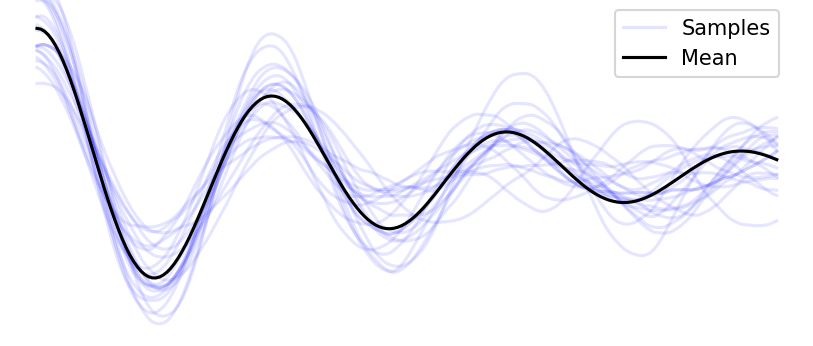
\includegraphics[width=\columnwidth]{../images/stochastic_spring_samples.png}
        \captionof{figure}{25 samples from the linear SDE describing the stochastic spring model with random independent force. The random force has $\sigma = 0.1$ and we have $k=1$, $l=0.2$.}
        \label{fig:spring_model}
    \end{center}
}

\subsection*{Discretizing the Prior in Time}
For a finite set of timesteps, the joint distribution of the finitely many states $\vec{U}(t)$ across timesteps becomes a multivariate Gaussian, as explored extensively in \cite{gp_Rasmussen}. In the spirit of the Method Of Lines (sec. \ref{sec:pde}), we will therefore consider a finite set of times $\mathbb{T} = \{0, h, 2h, 3h, \dots, T\}$, where $h$ is the timestep size and $T$ is the final time. For simplicity, we choose a fixed timestep, but it can be heterogenous or even adaptive, see \cite{nicoThesis}. 
\\
The Markov property then further enables the discrete time stochastic recurrence relation \cite{probnum} using eq. \ref{eq:SDE_mean} and \ref{eq:SDE_cov}
\begin{align}\label{eq:discrete_time_recurrence}
    \vec{U}(t+h) \;|\; \vec{u}(t) \sim \mathcal{N}(A\vec{u}(t), Q)
\end{align}
with discrete-time transition matrices
\begin{align}
    A &= e^{Fh}\label{eq:easy_matrix_exponential}
    \\
    Q &= \int_0^h e^{Ft}L\sigma^2L^\top e^{F^\top t} dt \label{eq:hard_matrix_exponential}
\end{align}
The formula \ref{eq:easy_matrix_exponential} can be computed numerically quite simply with JAX \cite{jax} or other numerical linear algebra libraries. \ref{eq:hard_matrix_exponential} is difficult, but using Matrix Fraction Decomposition it too can be reduced to a matrix exponential.
\definition{Matrix Fraction Decomposition}{
    The following algorithm for $A$ and $Q$ is adapted from \cite{sde-book} but simplified for our fixed-time-step and time-invariant case.
    \\
    Assume the SDE to be discretized is of the form as in eq. \ref{eq:LSDE_definition}. Compute the matrix exponential $M$ of the block-matrix
    $$M =\exp{\left(h\begin{bmatrix}
        F & \sigma^2LL^\top \\ 0 & -F^\top
    \end{bmatrix}\right)} \in \reals^{2n\times 2n}$$
    Extract the upper left block of $M$ as $A\in\reals^{n\times n}$ and the upper right as $C \in \reals^{n\times n}$. Finally, compute $Q$ as $Q = CA^\top$.
}
We can now form the conditional distribution of the state at each time given the state at the previous time. For brevity, we will from here on refer to as the discrete-time states $\vec{U}(i\cdot h)$ with integer subscript index $\vec{U}_i$. When combining the conditional distribution (eq. \ref{eq:discrete_time_recurrence}) with an initial Gaussian distribution 
$$\vec{U}_0 \sim \mathcal{N}(\mu_0, \Sigma_0)$$ 
we can form the factorized joint distribution of the process across all discrete times as 
$$P(\vec{u}_{\mathbb{T}}) = P(\vec{u}_0, \vec{u}_1, \dots, \vec{u}_{|T|}) =$$
$$\mathcal{N}\Big(\vec{u}_0;\;\mu_0, \Sigma_0\Big)\prod_{t=1}^{|\mathbb{T}|} \mathcal{N}\Big(\vec{u}_t;\;A\vec{u}_{t-1}, Q\Big)$$
This is an instance of a Linear Gaussian Model \cite{koller_bn}, which is a tractable and chain-structured Bayesian network \cite{pearl}, depicted below.
\begin{figure}[ht]
\begin{center}
    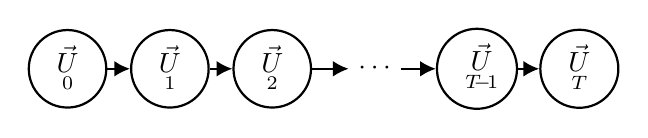
\begin{tikzpicture}[node distance=1.3cm, >={Latex[length=2mm, width=2mm]}, 
        obs/.style={circle, draw, align=center, text width = 3mm, minimum size=3mm, thick, font=\sffamily},
        lat/.style={rectangle, draw, align=center, text width = 6mm, minimum size=6mm, thick, font=\sffamily}]
        
        % Nodes
        \node[obs] (U0) {$\underset{0}{\vec{U}}$};
        \node[obs, right of=U0] (U1) {$\underset{1}{\vec{U}}$};
        \node[obs, right of=U1] (U2) {$\underset{2}{\vec{U}}$};
        \node[right of=U2] (dots) {$\cdots$};
        \node[obs, right of=dots] (UTb) {$\underset{T\!\!-\!1}{\vec{U}}$};
        \node[obs, right of=UTb] (UT) {$\underset{T}{\vec{U}}$};
        
        % Edges
        \draw[->, thick] (U0) -- (U1);
        \draw[->, thick] (U1) -- (U2);
        \draw[->, thick] (U2) -- (dots);
        \draw[->, thick] (dots) -- (UTb);
        \draw[->, thick] (UTb) -- (UT);
    \end{tikzpicture}
\end{center}
\caption{The Bayesian network of the discrete-time states $\vec{U}_i$.}
\label{fig:finite_time_states}
\end{figure}
\subsection*{Using the distribution as a Prior}
To use the discrete-time distribution of functions as a prior distribution, we need to integrate further information into the system that we can then update the prior with. We will extend the Bayesian network with potential observations $O_i$ of each state $\vec{U}_i$. Although we might not know the complete state at each instant, there might be properties that we do know, such as the derivative of the function at some time. 
\\ To build on the network in fig. \ref{fig:finite_time_states}, we will define the conditional distributions of a partial observations of some of the time instances. These partial observations at time $i$ are expressed as $O_i \sim \mathcal{N}(m(\vec{U}_i), \Sigma_m)$, where $m$ is an affine\footnote{The measurement model has to be a linear function of the state, as the joint distribution will only be multivariate Gaussian under linear transformations.} function of $\vec{U}_i$. $m$ will be thought of as a measurement model, although this interpretation can bring along physical assumptions that are not always helpful. We will usually have $\Sigma_m = \mathbf{0}$\footnote{This case is reffered to as the "Dirac Likelihood" \cite{exponential_probabilistic} because it places all mass on a single event.}, but nonzero noise can be useful, as in \cite{pnmol}\footnote{Here, the authors use it to model uncertainty in the ODE description itself, which can stem from coarse discretization of an underlying PDE or from left out terms}.
Each $O_i$ is a function of only the state $\vec{U}_i$, and so the extended Bayesian Network takes the following form
\begin{figure}[ht]
    \centering
        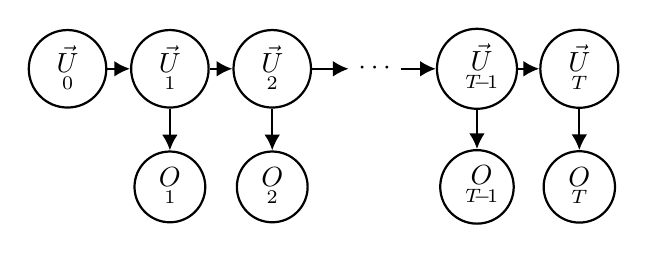
\begin{tikzpicture}[node distance=1.3cm, >={Latex[length=2mm, width=2mm]}, 
            obs/.style={circle, draw, align=center, text width = 3mm, minimum size=3mm, thick, font=\sffamily},
            lat/.style={rectangle, draw, align=center, text width = 6mm, minimum size=6mm, thick, font=\sffamily}]
            
            % Nodes
            \node[obs] (U0) {$\underset{0}{\vec{U}}$};
            \node[obs, right of=U0] (U1) {$\underset{1}{\vec{U}}$};
            \node[obs, right of=U1] (U2) {$\underset{2}{\vec{U}}$};
            \node[right of=U2] (dots) {$\cdots$};
            \node[obs, right of=dots] (UTb) {$\underset{T\!\!-\!1}{\vec{U}}$};
            \node[obs, right of=UTb] (UT) {$\underset{T}{\vec{U}}$};
            
            \node[obs, below of=U1, yshift=-0.2cm] (O1) {$\underset{1}{O}$};
        \node[obs, below of=U2, yshift=-0.2cm] (O2) {$\underset{2}{O}$};
        \node[obs, below of=UTb, yshift=-0.2cm] (OTb) {$\underset{T\!\!-\!1}{O}$};
        \node[obs, below of=UT, yshift=-0.2cm] (OT) {$\underset{T}{O}$};
        
        % Edges
        \draw[->, thick] (U0) -- (U1);
        \draw[->, thick] (U1) -- (U2);
        \draw[->, thick] (U2) -- (dots);
        \draw[->, thick] (dots) -- (UTb);
        \draw[->, thick] (UTb) -- (UT);
        
        \draw[->, thick] (U1) -- (O1);
        \draw[->, thick] (U2) -- (O2);
        \draw[->, thick] (UTb) -- (OTb);
        \draw[->, thick] (UT) -- (OT);    
    \end{tikzpicture}
    \caption{The full Bayesian network we will be working with. $\vec{U}_0$ must be provided, and one can then condition on values of some or all observations $O_i$.}
    \label{fig:full_bayesian_network}
\end{figure}

The specific choice of measurement model will depend on the problem. It can abstractly be modeled as the Information Operator.
\definition{Information Operator}{
    The Information Operator (\cite{information_operator}) is a measurement model that maps specific functions of interest to zero. Zero is an arbitrary choice made for convenience, it could have been any other number. Information operators are generally not affine, but they can, using the Jacobian, be linearized around the predicted mean of the unobserved state with a first order Taylor approximation. This is a topic for the Kalman Filter section.
}
To get a sense of the usual prior distributions used in probabilistic numerical solvers, we will introduce two common choices, the Integrated Wiener process, and the Integrated Ornstein-Uhlenbeck process.
\definition{Integrated Wiener Process}{
    \begin{center}
        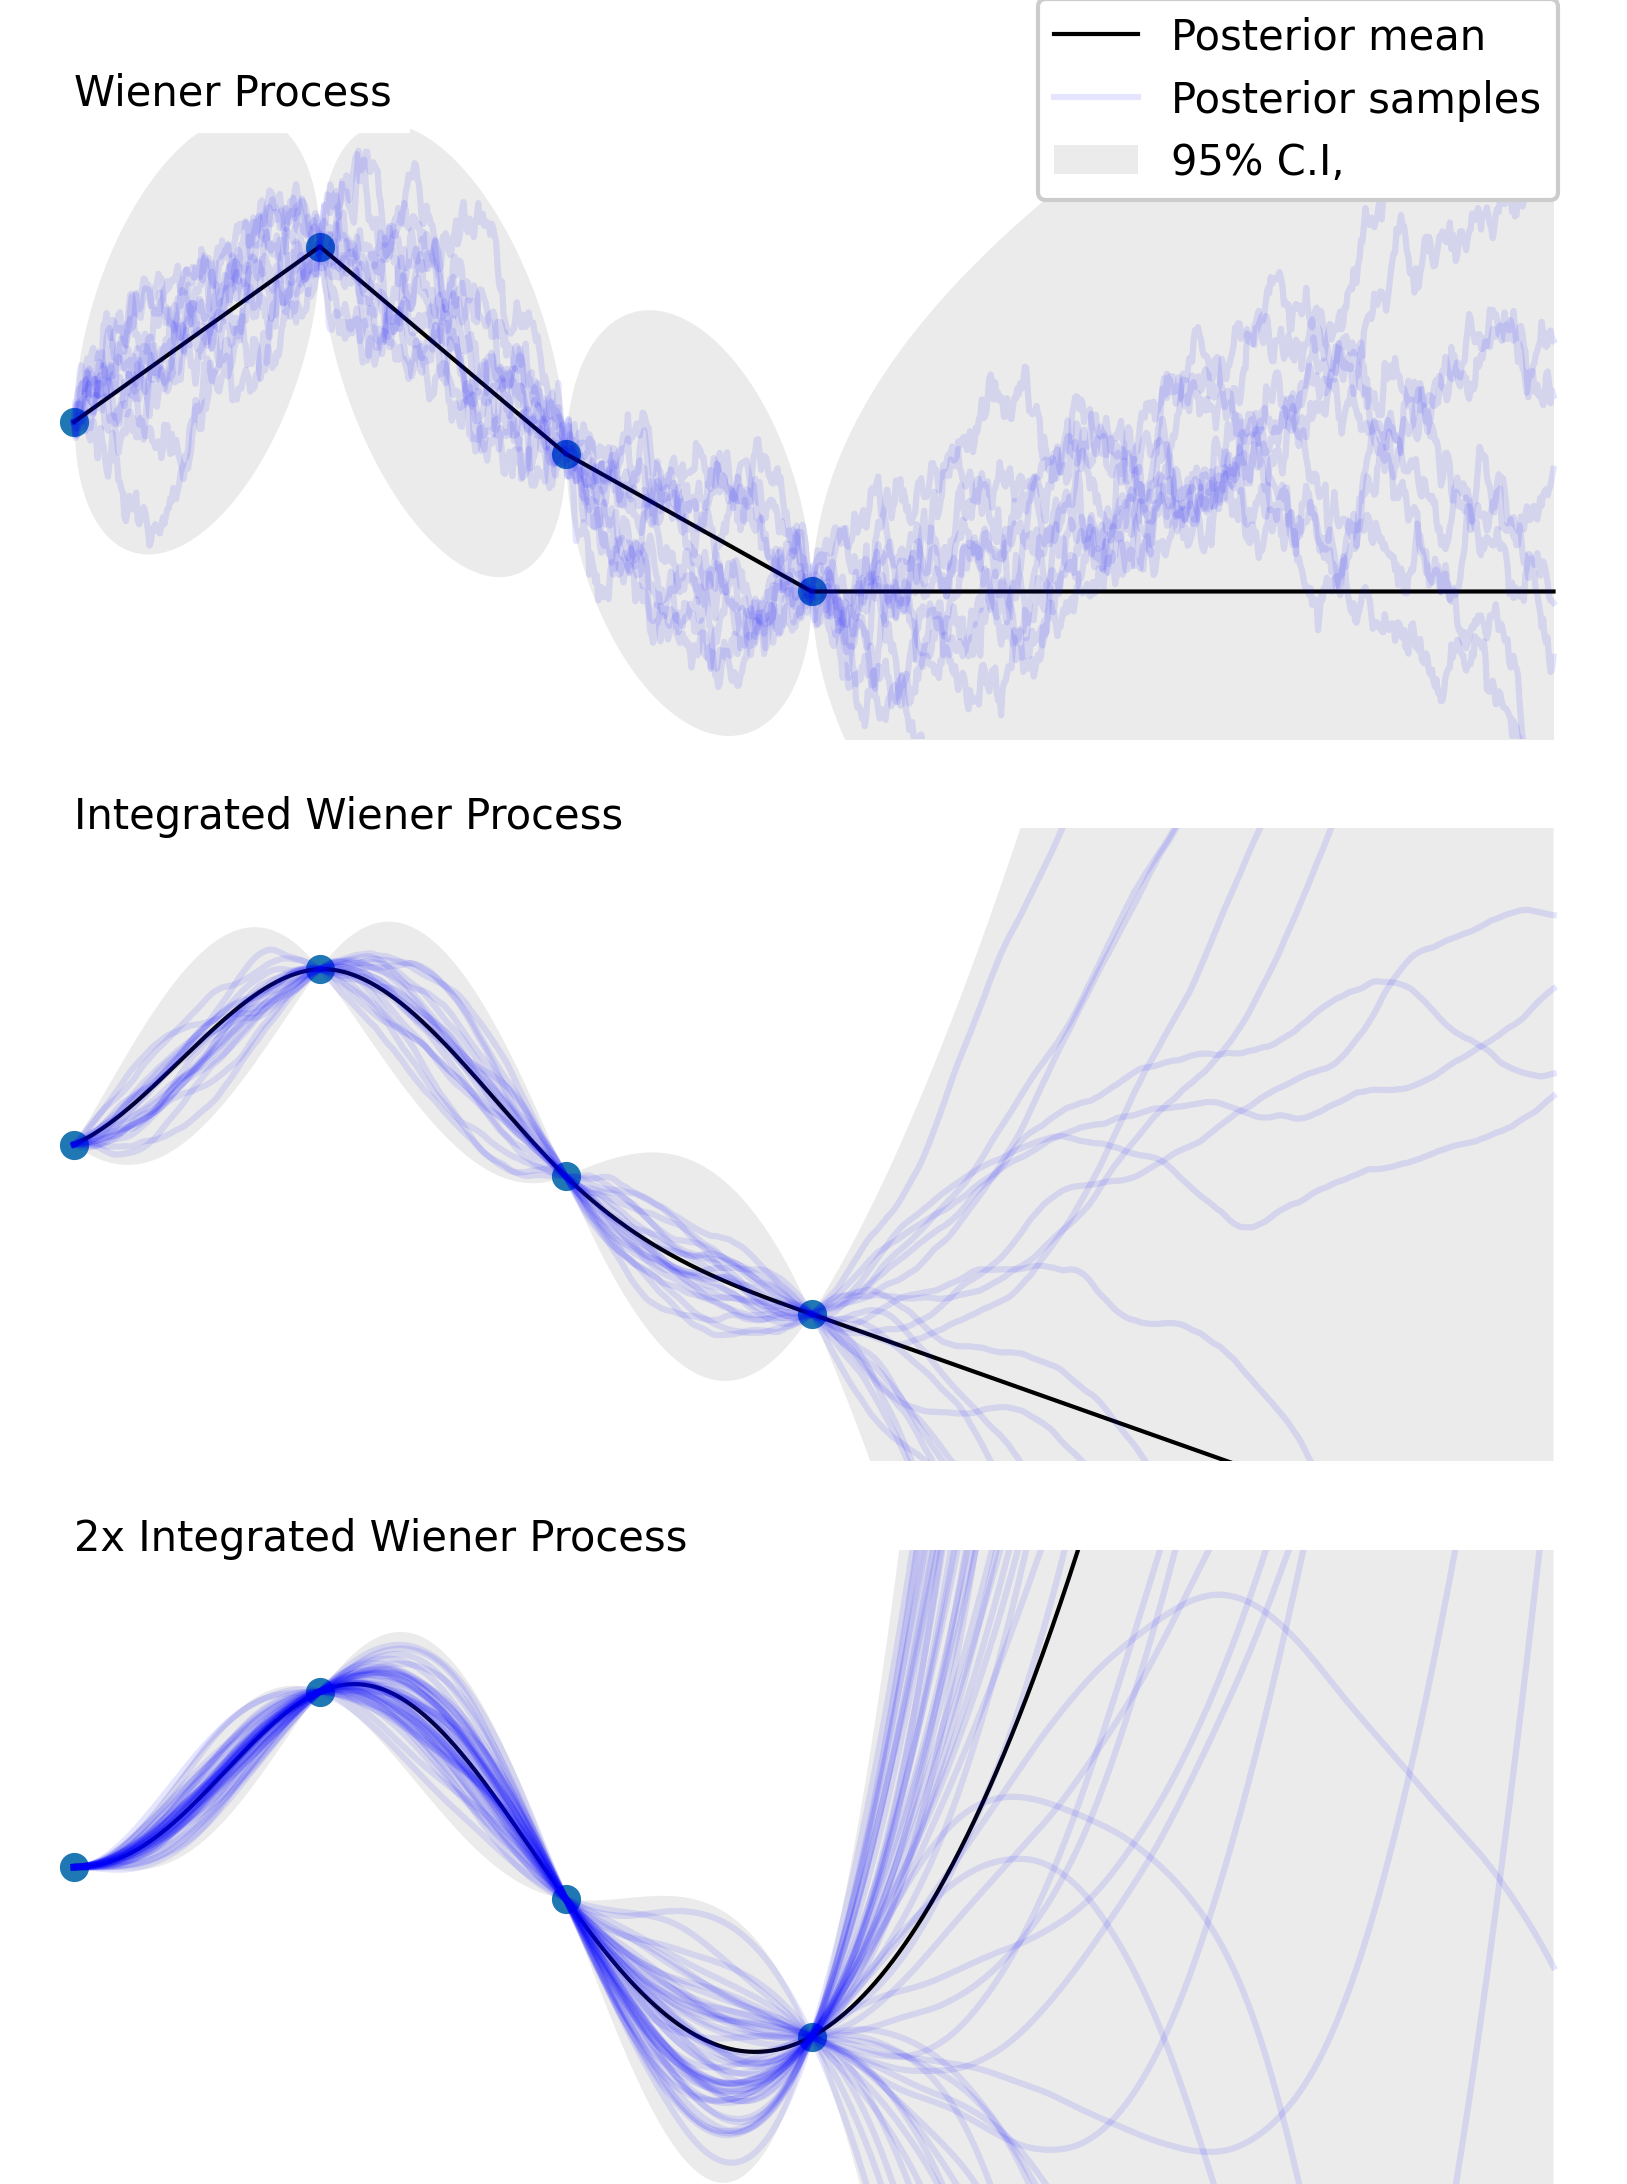
\includegraphics[width=\columnwidth]{../images/conditioned_iwps.png}
        \captionof{figure}{Three graphs of the [x-Integrated] Wiener Process. The processes are conditioned to pass through four different points, marked in blue, the derivative is however unspecified.}
        \label{fig:iwps}
    \end{center}
    The Wiener Process, also known as Brownian motion, is continuous but nowhere differentiable. In terms of eq. \ref{eq:LSDE_definition} its state-space representation is 1-dimensional with $$F=0  \hspace{1cm}L=1$$ 
    The Integrated Wiener Process is the integral of the Wiener Process. The state-space representation is 2-dimensional with $$F=\begin{bmatrix}
        0 & 1 \\ 0 & 0
    \end{bmatrix} \hspace{1cm} L=\begin{bmatrix}
        0 \\ 
        1 
    \end{bmatrix}$$
    \\ The Twice Integrated Wiener Process has 3-dimensional state-space with $$F=\begin{bmatrix}
        0 & 1 & 0 \\ 0 & 0 & 1 \\ 0 & 0 & 0
    \end{bmatrix} \hspace{1cm} L=\begin{bmatrix}
        0 \\ 0 \\ 1
    \end{bmatrix}$$
    \\ The posterior means of the $q$-times integrated Wiener process are 2q + 1-ic splines (\cite{probnum}) - see the figure above. There is in principle nothing preventing us from using higher order integrated Wiener processes, but numerical issues can be encountered already at $q=3$. We will tackle this later.
}
\definition{Ornstein Uhlenbeck Process}{
    \begin{center}
        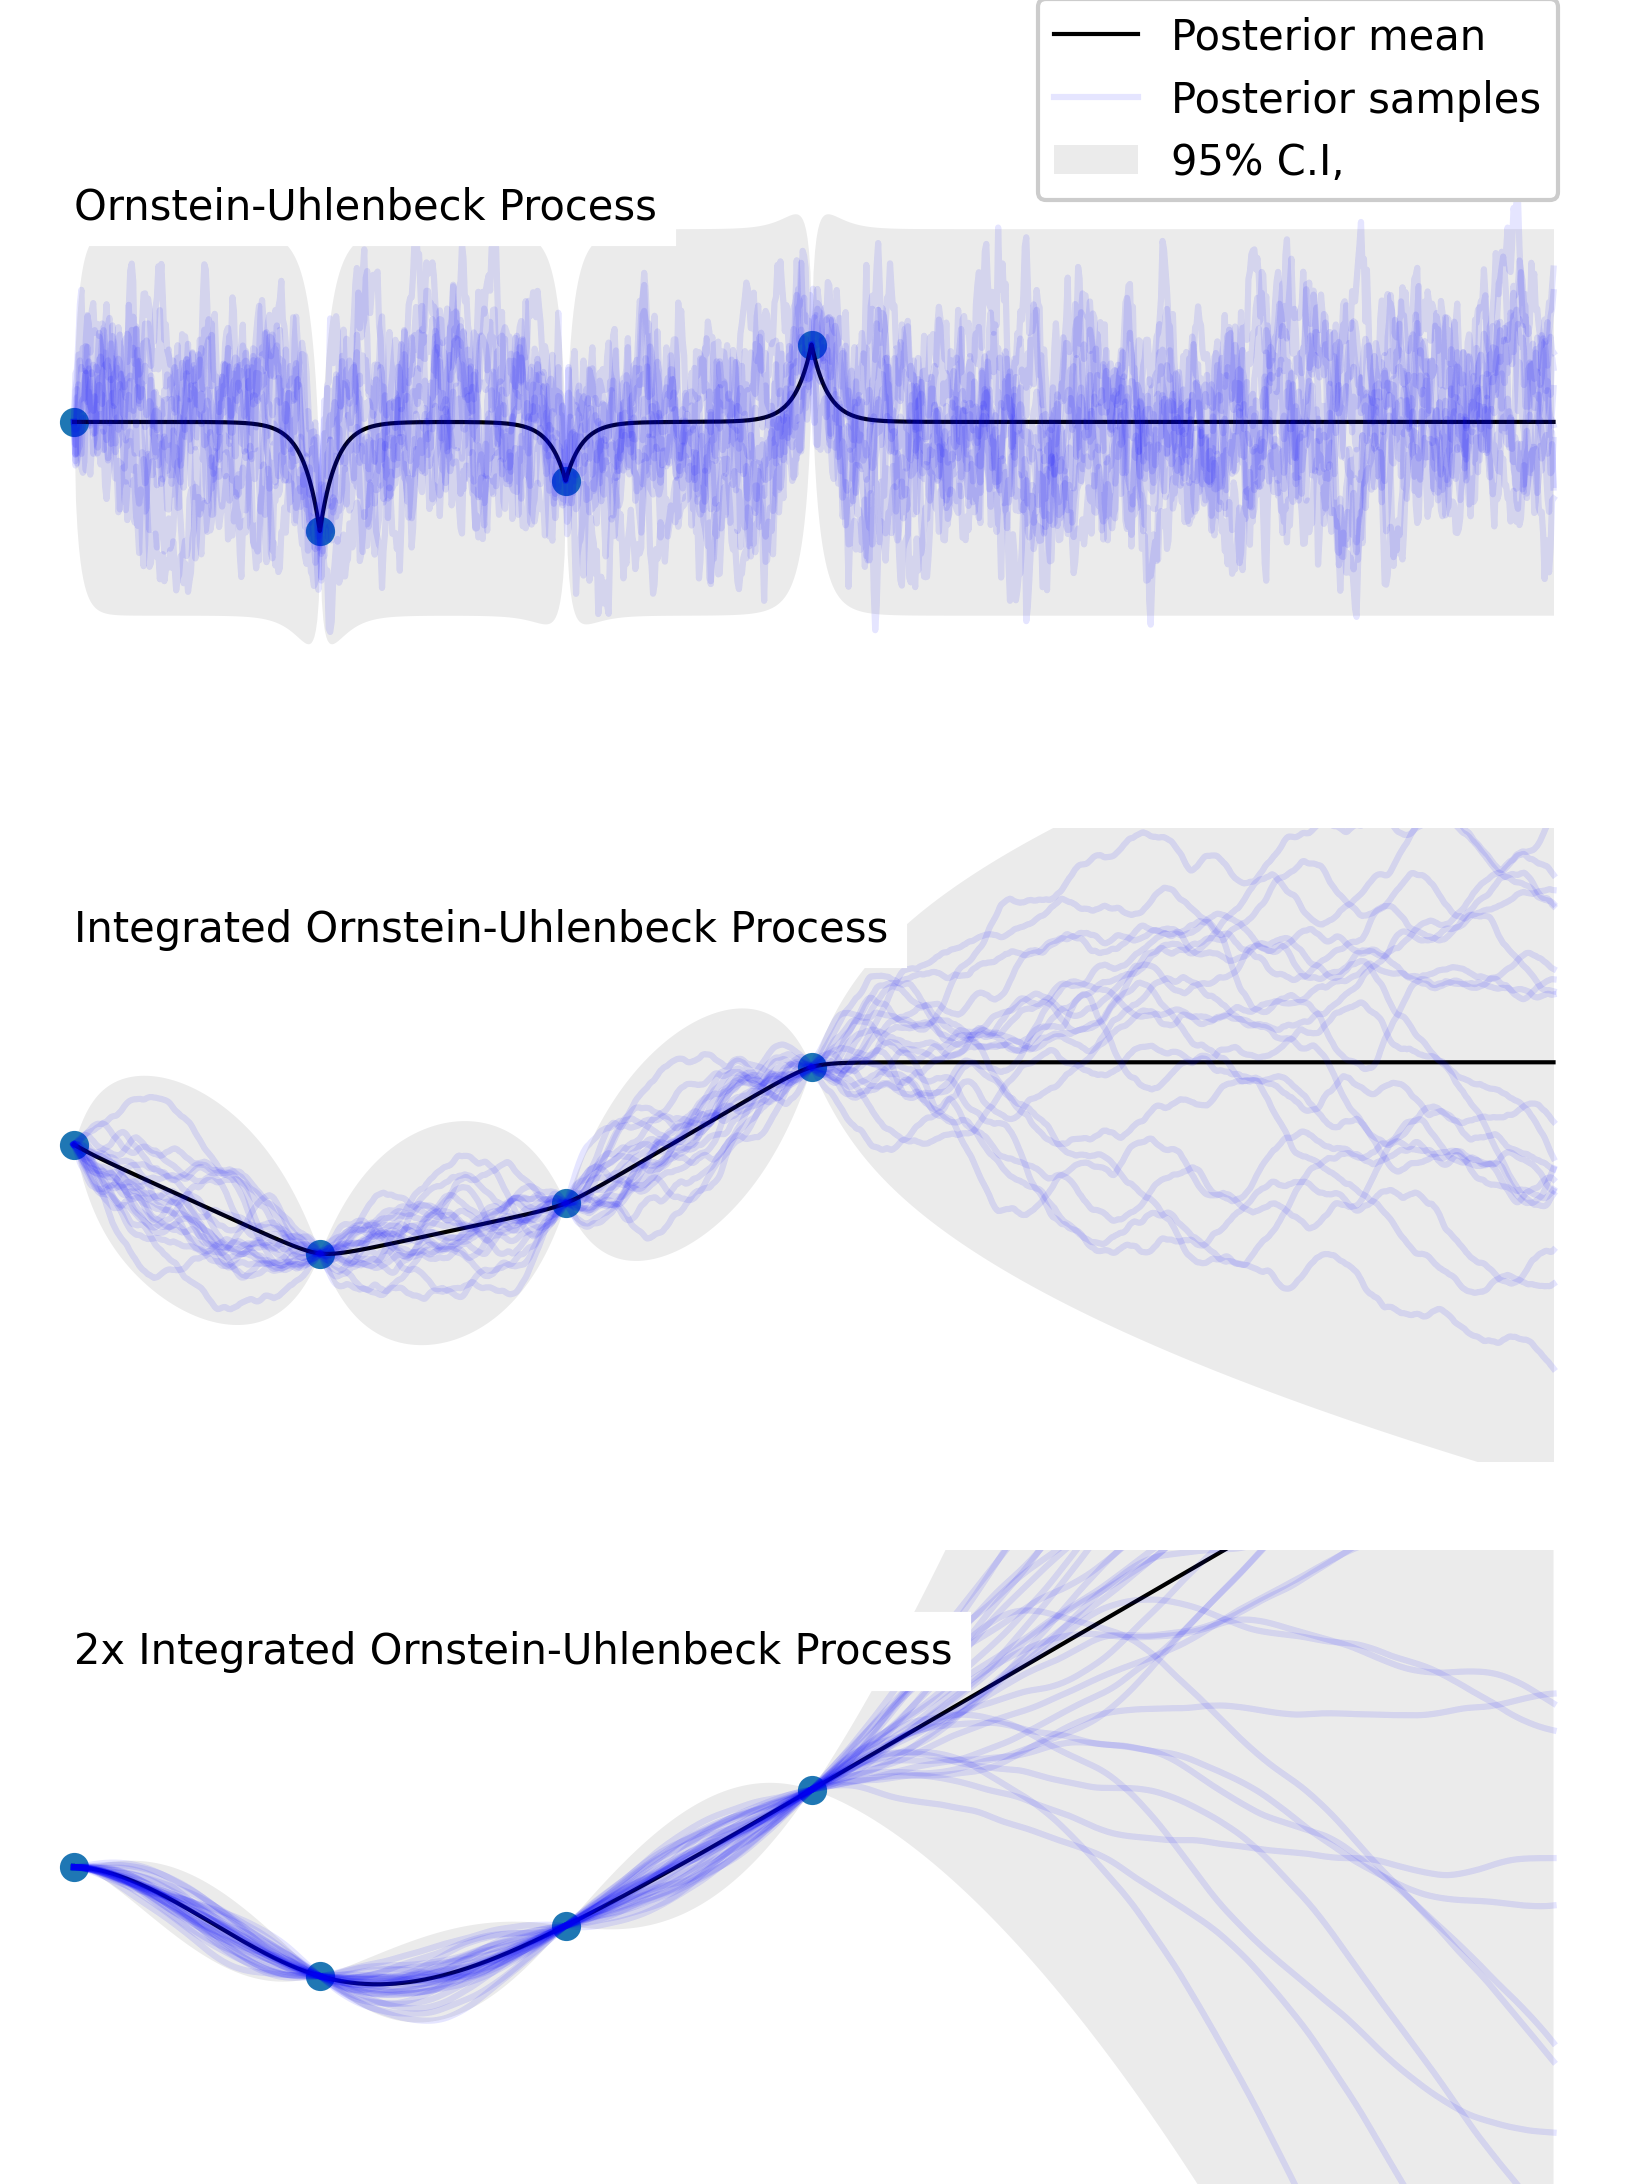
\includegraphics[width=\columnwidth]{../images/conditioned_ous.png}
        \captionof{figure}{Draws from the Integrated Wiener Process, Conditioned}
        \label{fig:ous}
    \end{center}
    The Ornstein-Uhlenbeck Process depends on rate parameter $a>0$. In terms of eq. \ref{eq:LSDE_definition} its state-space representation is 1-dimensional with $$F=-a  \hspace{1cm}L=1$$ 
    The Integrated Ornstein-Uhlenbeck is the integral of the Ornstein-Uhlenbeck. The state-space representation is 2-dimensional with $$F=\begin{bmatrix}
        0 & 1 \\ 0 & -a
    \end{bmatrix} \hspace{1cm} L=\begin{bmatrix}
        0 \\ 1
    \end{bmatrix}$$
    \\ The Twice Integrated Ornstein-Uhlenbeck has 3-dimensional state-space with $$F=\begin{bmatrix}
        0 & 1 & 0 \\ 0 & 0 & 1 \\ 0 & 0 & -a
    \end{bmatrix} \hspace{1cm} L=\begin{bmatrix}
         0 \\ 0 \\  1
    \end{bmatrix}$$
    In \cite{exponential_probabilistic} they suggest using the Ornstein-Uhlenbeck process to encode prior information to solve particularly difficult "stiff" DEs.\\
    The Ornstein-Uhlenbeck process is mean-reverting (\cite{probnum}), the derivative of the Integrated Ornstein-Uhlenbeck reverts to zero, and the curvature of the Twice Integrated Ornstein-Uhlenbeck reverts to zero.
}
Defining the state projection matrices will be helpful for notation. They appear commonly in the literature on probabilistic numerical solvers.
\definition{State Projection Matrices $E_q$}{
    We want an convenient way of selecting a specific order derivative $q$ from the state $\vec{U}_i \in \reals^{n\cdot (1+q)}$. We can do so by projecting the full state onto the $q$-th derivative with the projection matrices $E_q\in\reals^{n \times n\cdot (1+q)}$, which are block matrices
    \begin{align*}
        E_0 &= \begin{bmatrix}
            \textbf{I}_n & \textbf{0} & \cdots & \cdots & \textbf{0}
        \end{bmatrix}
        \\
        E_1 &= \begin{bmatrix}
            \textbf{0} & \textbf{I}_n & \textbf{0} & \cdots & \textbf{0}
        \end{bmatrix}
        \\
        &\dots
        \\
        E_q &= \begin{bmatrix}
            \textbf{0} & \cdots & \cdots & \textbf{0} & \textbf{I}_n
        \end{bmatrix}
    \end{align*}
    They have the property that $E_q \vec{U} = \frac{d^q}{d t^q} U$ and that they are linear transformations.
}

\definition{ODE Residual Measurement Function}{
    An instance of an Information Operator that we will make heavy use of is the ODE residual measurement function. It will map all functions that satisfy the ODE to zero.
    For an example linear ODE $$\frac{d^2}{dt^2}U(t) = AU(t)$$ it is defined as 
    $$\mathcal{R}\vec{U}(t) = E_2\vec{U}(t) - AE_0\vec{U}(t) \in \reals^n$$ which is expressing residual of the ODE in terms of the state-space representation. A solution of the ODE will have $\mathcal{R}\vec{U}(t) = \mathbf{0}$.
}
If definition of $\mathcal{R}\vec{U}(t)$ refers to some derivative $E_q$, then the prior distribution must model at least $q$ derivatives for it to be defined. By conditioning the prior residual of $\mathcal{R}\vec{U}(t)$ to be zero at all times $t \in \mathbb{T}$, we are "weeding out" the functions that surely do not satisfy the ODE, forcing the state-space representation of the function to satisfy the ODE. The associated observation model with the residual operator as measurement function is deterministic and given as $$O_i \sim \mathcal{N}(E_2\vec{U}(t) - AE_0\vec{U}(t), \Sigma_h)$$
\\
The residual operator can be used to encode linear \textit{PDEs} as well:
\example{More examples of Residual Measurement for PDEs}{
    One can also encode PDEs with the residual operator by first converting it to an ODE using the method of lines. We will convert the examples from section \ref{sec:pde}. 
    \begin{center}
    \begin{tabular}{c|c}
        \hline 
        Linear PDE & $\mathcal{R}\vec{U}$
        \\\hline \hspace*{2mm} & \hspace*{2mm} 

        % START
        \\$\frac{\partial}{\partial t}u = -\Delta u$ & $E_1\vec{U} + dLE_0\vec{U}$
        \\ \hspace*{2mm} & \hspace*{2mm} 
        % END
        
        % START
        \\\hline \hspace*{2mm} & \hspace*{2mm} 
        \\$\frac{\partial^2}{\partial t^2}u = ku  -d\Delta \frac{\partial}{\partial t}u$ & $E_2\vec{U} - kE_0\vec{U} + dLE_1\vec{U}$
        \\ \hspace*{2mm} & \hspace*{2mm} 
        % END
        
        % START
        \\\hline \hspace*{2mm} & \hspace*{2mm} 
        \\$\frac{\partial^2}{\partial t^2}u = a\Delta \frac{\partial}{\partial t}u$ & $E_2\vec{U} - aE_1\vec{U}$
        \\ \hspace*{2mm} & \hspace*{2mm} 
        % END

        % START
        \\\hline \hspace*{2mm} & \hspace*{2mm} 
        \\$\frac{\partial^3}{\partial t^3}u = \Delta u$
        & $E_3\vec{U} - LE_0\vec{U}$
        \\ \hspace*{2mm} & \hspace*{2mm} 
        % END

        % START
        \\\hline \hspace*{2mm} & \hspace*{2mm} 
        \\$\frac{\partial^4}{\partial t^4}u = \Delta u + a\frac{\partial^2}{\partial t^2}u $ & 
        $E_4\vec{U} - LE_0\vec{U} - aE_2\vec{U}$
        \\ \hspace*{2mm} & \hspace*{2mm} 
        \\\hline
        % END
    \end{tabular}
    \end{center}
}

\example{Function Values at specific times}{
    How did we generate the figures in fig.\ref{fig:iwps} and get the posterior to pass through the initial four points? For the twice integrated scalar Wiener Process, we choose an initial distribution $\vec{U}(0) \sim \mathcal{N}(\mathbf{0}^3, \mathbf{0}^{3 \times 3})$ and define the affine observation function $h(\vec{U}_i) = E_0\vec{U}_i \in \reals$ with $E_0 = [1 \;\; 0 \;\; 0]^\top$. 
    \\
    The four blue points $P_t \in \reals$ at times $t\in\{0, \frac{1T}{8}, \frac{2T}{8}, \frac{3T}{8}\}$ are reflected in the posterior by conditioning the prior on the data points $E_0\vec{U}_t = P_t$. The posterior will then pass through these points. The derivative is however not specified, and which lets the prior "speak" and impose regularity \footnote{$C^2$ regularity for the twice integrated Wiener Process}. 
}
We have so far postponed the actual task of computing the posterior. This is what we will cover now.
\subsection*{Kalman Filter and Rauch-Tung-Striebel Smoother}
The sparse connections of the Gaussian Bayesian network in fig. \ref{fig:full_bayesian_network} can be exploited. Together, the Kalman Filter and RTS Smoother form a message passing algorithm (\cite{koller_bn}) for computing the conditional distribution of linear Gaussian models. 
The chain-structure allows for a very efficient ordering of the messages, going from $i=0$ to $i=|T|$ in a forward pass and from $i=|T|$ to $i=1$ in a backward pass. 
% If one were to form the full joint distribution as mean-vector $\mu$ and covariance matrix, the cost of computing the posterior would be of order $O(|\mathbb{T}|^3n^3)$ by the cubic cost of matrix inversion required for the covariance matrix.
\definition{Forward Pass, Kalman Filter}{
    The Kalman Filter \cite{kalman} computes, for a linear Gaussian graphical model like in fig. \ref{fig:full_bayesian_network} and observations $o_i$ (for all or some $i$), the distribution 
    \begin{align}\label{eq:kalman_forward_pass}
        p\left(\vec{U}_i \;\Big|\; o_{1:i}\right) \hspace{5mm} i\in\{1, \dots, |\mathbb{T}|\}
    \end{align}
    in increasing order of $i$. This is the posterior distribution of each state, given all observations up to that time. These distributions have no knowledge of future information. However, eq. \ref{eq:kalman_forward_pass} includes the terminal time distribution, 
    \begin{align}
        p\left(\vec{U}_{|\mathbb{T}|} \;\Big|\; o_{1:|\mathbb{T}|}\right)\label{eq:terminal_time_posterior}
    \end{align}
    which is the posterior of the final state given information about \textit{all} the observations (since there are no future observations). If one is interested only in the posterior at the final time, then the Kalman Filter forward pass is enough. 
}
The term "filter" refers to accumulating [uncertain] information about past states into some estimate of the current state. An exponential moving average is also a filter.
\example{Choosing the noise scale $\sigma^2$}{
    In our definition of the prior LTI SDE, we left the parameter $\sigma$ unspecified. This parameter is the noise scale, and it is a hyperparameter that must be chosen. \cite{nicoThesis} derives a maximum likelihood estimate of $\sigma$, which can be computed cheaply during the forward pass. The issues of hand-tuning $\sigma$ are therefore mitigated, and the $\sigma$ that maximises the probability of the observations is chosen. Our implementation uses this method.
}

\definition{Backward Pass, Rauch-Tung-Striebel Smoother}{
    The RTS smoother \cite{rts} runs a backward pass that computes the full posterior distribution of the states, given the output from the Kalman filter forward pass.
    \begin{align}\label{eq:kalman_forward_pass}
        p\left(\vec{U}_i \;\Big|\; o_{1:|\mathbb{T}|}\right) \hspace{5mm} i\in\{|T|, \dots, 0\}
    \end{align}
    This is the marginal posterior distribution of each state, given all observations.
}
\example{Sampling the Posterior}{
    The forward pass can additionally produce the "backwards" conditional distributions
    $$p\left(\vec{U}_{i} \;\Big|\; \vec{U}_{i+1}, o_{1:i}\right)$$ which defines a chain-structured Bayesian network like fig \ref{fig:finite_time_states}, with the arrows pointing in the reverse direction. One can then use ancestral sampling, starting with a sample from \ref{eq:terminal_time_posterior} and sampling from the backwards distributions to get a sample from the full posterior. Ancestral sampling involves iterating through the states in the backwards direction, and is thus best left for the backward pass. This is how we draw posterior sample in figures \ref{fig:iwps} and \ref{fig:ous}.
}
After a forwards and backwards pass, all information about the observations $O_i$ has reached every state, which ensure that the final distribution reflects the posterior distribtution given all observations, not just the preceding observations.
\\
Together, they facilitate computing the posterior in time $O(|\mathbb{T}|n^3)$ (\cite{invention_of_ODE_solver}), where $n$ is the size of the state. Note the linear dependence on amount of timesteps, which is also present in classical numerical solvers (\cite{probnum}). It is remarkable that the same can be achieved while additionally modeling the full posterior distribution. 
\\
We mention that the measurement function has to be linear, and therefore kept the examples of the information operator linear as well. To break free from the restraints of linear PDEs, we will make use of the Extended Kalman Filter forward pass. 
\definition{Forward Pass, Extended Kalman Filter}{
    The Extended Kalman Filter is used extensively in robotics and control \cite{probnum}, but is also applicable for nonlinear PDEs (\cite{nicoThesis}, \cite{information_operator}), which are arguably the more interesting case.\\
    As mentioned, the observation model is of the form 
    $$O_i \;|\; \vec{u}_i \sim \mathcal{N}(m(\vec{u}_i), \Sigma_m)$$
    and requires an affine $m$. For a nonlinear measurement function $n$, we will adaptively update $n$ to be affine during the forward pass by Taylor-expanding it around the most recent believed mean of state $\vec{U}_i$, $\bar{u_i} = \mathbb{E}[\vec{U}_i \;|\; o_{1:{i-1}}]$\footnote{This conditional distribution is obtained by applying eq. \ref{eq:discrete_time_recurrence} with eq. \ref{eq:kalman_forward_pass} and marginalizing.}. The Taylor approximation of $n$ at time $i$ becomes 
    $$\bar{n_i}(u) = n(\bar{u_i}) + J(\bar{u_i})(y) - J(n)(\bar{u})$$ 
    with $J$ the Jacobian matrix of $n$. It will be the most accurate around the prior mean. With this adaptive measurement function defined, one can use the classic forward Kalman filter forward pass with the conditional distribution
    $$O_i \;|\; \vec{u}_i \sim \mathcal{N}((\bar{n_i}(\vec{u}_i)), \Sigma_m)$$
    \\
    Because we can linearize the (assumed to be differentiable) Information operator, we can more generally define the residual measurement $\mathcal{R}\vec{U}(t)$ for a nonlinear PDEs $$\frac{\partial^q}{\partial t^q}u = f(u)$$ as the nonlinear measurement function $$\mathcal{R}\vec{U}(t) = E_q\vec{U}(t) - f\left(\vec{U}(t)\right)$$ The Extended Kalman filter then takes care of interpreting this as an affine function of the state using automatic differentiation.
}
\subsubsection*{More Implementation Details}
We implement our solver in JAX \cite{jax}, which is a Python library for automatic differentiation and high performance numerical linear algebra. It further allows just-in-time compilation of functional programs, which greatly speeds up all procedures by vectorizing and parallelizing where possible. With 64-bit floating point precision, one might hope that the numerical stability of the solver would not an issue. However, the covariance matrices that are formed in the Kalman Filter and RTS Smoother can have very poor condition numbers, which can lead to numerical instability. The covariance matrix generally stores entries that are the square of the length-scale of the state. For small timesteps, the standard deviation in the conditional distribution between states will be small, and the covariance matrix in \ref{eq:hard_matrix_exponential} will contain the square of this small number. This can lead to vanishingly small entries in the covariance matrix that worsen the condition number. \\
\textit{"Roughly speaking, the condition number states how much precision is lost when inverting a matrix and the larger the number, the more precision is lost. Huge condition numbers render the solution of linear systems practically infeasible."} - from \cite{nicoThesis}

\definition{Improving Numerical Stability, generalized Cholesky factors}{
In \cite{nicoThesis} they suggest using generalized Cholesky factors \cite{choleskyQR} of the covariance matrix to improve numerical stability. Generalized Cholesky Factors always exist for symmetric, positive semidefinite matrices\footnote{The covariance matrices are usually positive definite, but it will be semidefinite when some part of state is deterministic.}. A covariance matrix $\Sigma\in \reals^{n \times n}$ can be factored as $\Sigma =  CC^\top$ where $C = \Sigma^{(1/2)} \in \reals^{n\times n}$ is a lower triangular matrix. A multivariate Gaussian distribution is then parameterized by a mean vector and the generalized Cholesky factor of the covariance matrix. 
\\
\cite{nicoThesis} give the full description of how, given a Cholesky parameterization of $X \sim \mathcal{N}(x; Ax + b, \Sigma)$ and $Y \;\big|\; X=x \sim \mathcal{N}(y; Cx + d, \Sigma)$, one can compute the posterior $P(X | Y)$, marginal $P(Y)$ and the likelihood $P(Y | X)$ in closed form, all without having to form the covariance matrix. This sidesteps the numerical instability of the covariance matrix.
}\noindent
As an approximation, using generalized Cholesky factors representation allowed us to take $\times 1.5$ more steps with the solver before numerical instability invalidated the results. It however turns out that the covariance matrix is still ill-conditioned due to an orthogonal issue. The matrix $Q$ depends still on the step-size $h$ in \ref{eq:hard_matrix_exponential}. In the case of the integrated Wiener process, for $q$ derivatives, the condition number grows at least as $2^q$ an in practice is worse for low $h$, yielding entries down to $10^{-40}$ for $q=3, h=0.0001$ (\cite{nicoThesis}). 
\definition{Improving Numerical Stability, Preconditioning}{
    As argued and solved in \cite{nicoThesis}, $Q$ should not depend on the length of the time step. They give an invertible linear coordinate transformation $T$ to the SDE, which will remove this dependency. Because we are working with LTI SDEs, this transformation can be applied at the SDE level to the matrices as $TFT^{-1}$ and $TLL^\top$. It can then be undone at the end of the backward pass to get the posterior in the original state-space.
    \\
    The transformation is derived for the integrated Wiener process, but when implementing it in the thesis and applying it to other LTI SDEs we were still able to model up to 10 derivatives in all processes instead of the previous 3. This is a significant improvement and unlocks the possibility of using higher order integrated processes.
}
The first state and derivatives can be informed by the vector field $f$ - if the DE is of the form $\frac{d}{dt}u = f(u)$, we immediately get the expression for the first derivative as $f(u(0))$. If however the DE is of the from $\frac{d^2}{dt^2}u = f(u)$, we cannot extract the initial derivative, and it is considered in input value, like the initial value $u(0)$. As will also be explored further in chapter \ref{sec:solver_experiments}, one can repeatedly differentiate the vector field to get further derivatives of the initial state.\\
\definition{Initialization, Taylor-mode automatic differentiation}{
    If using automatic differentiation, one first has to compute the Jacobian, then the Hessian and so on for higher derivatives. The complexity of this grows exponentially with the order of the derivative as $O(2^q)$ \cite{nicoThesis}. Instead they propose using Taylor-mode automatic differentiation \cite{taylor_mode}, \cite{taylor_mode_jax} to get the higher derivatives w.r.t. time, which grows as $O(\exp(\sqrt{q}))$. Our implementation uses Taylor-mode automatic differentiation function from Python library \texttt{probdiffeq} \cite{nicoThesis} to initialize the higher derivatives for the experiments to come. 
}
\newpage
\example{Solving the Damped Harmonic Oscillator}{

    Finally, we want to give an example of a solving the damped harmonic oscillator with our probabilistic numerical solver. We solve the ODE $$\frac{d^2}{dt^2}u = -0.3\frac{d}{dt}u - 1.5u$$ with initial conditions $u(0) = 1$ and $\frac{d}{dt}u(0) = 0$.
    \\
    We show the posterior distribution of the 4-times integrated Wiener process after being initialized using Taylor-mode automatic differentiation and conditioning on the PDE residual 
    $$\mathcal{R}(\vec{U}) = \vec{U}_2 + 0.3\vec{U}_1 + 1.5\vec{U}_0$$
    of the damped harmonic oscillator being zero. To show the effect of using a higher order integrated prior, we condition only at five timesteps, show as blue dots\footnote{The vertical position of the blue dots has no meaning and is arbitrarily placed on the mean of the process. We are \textit{not} conditioning the process to pass through these points, unlike in figures \ref{fig:iwps}}. The true solution is shown in red and is computed using the matrix exponential (eq. \ref{eq:matrix_exp}).
    \begin{center}
        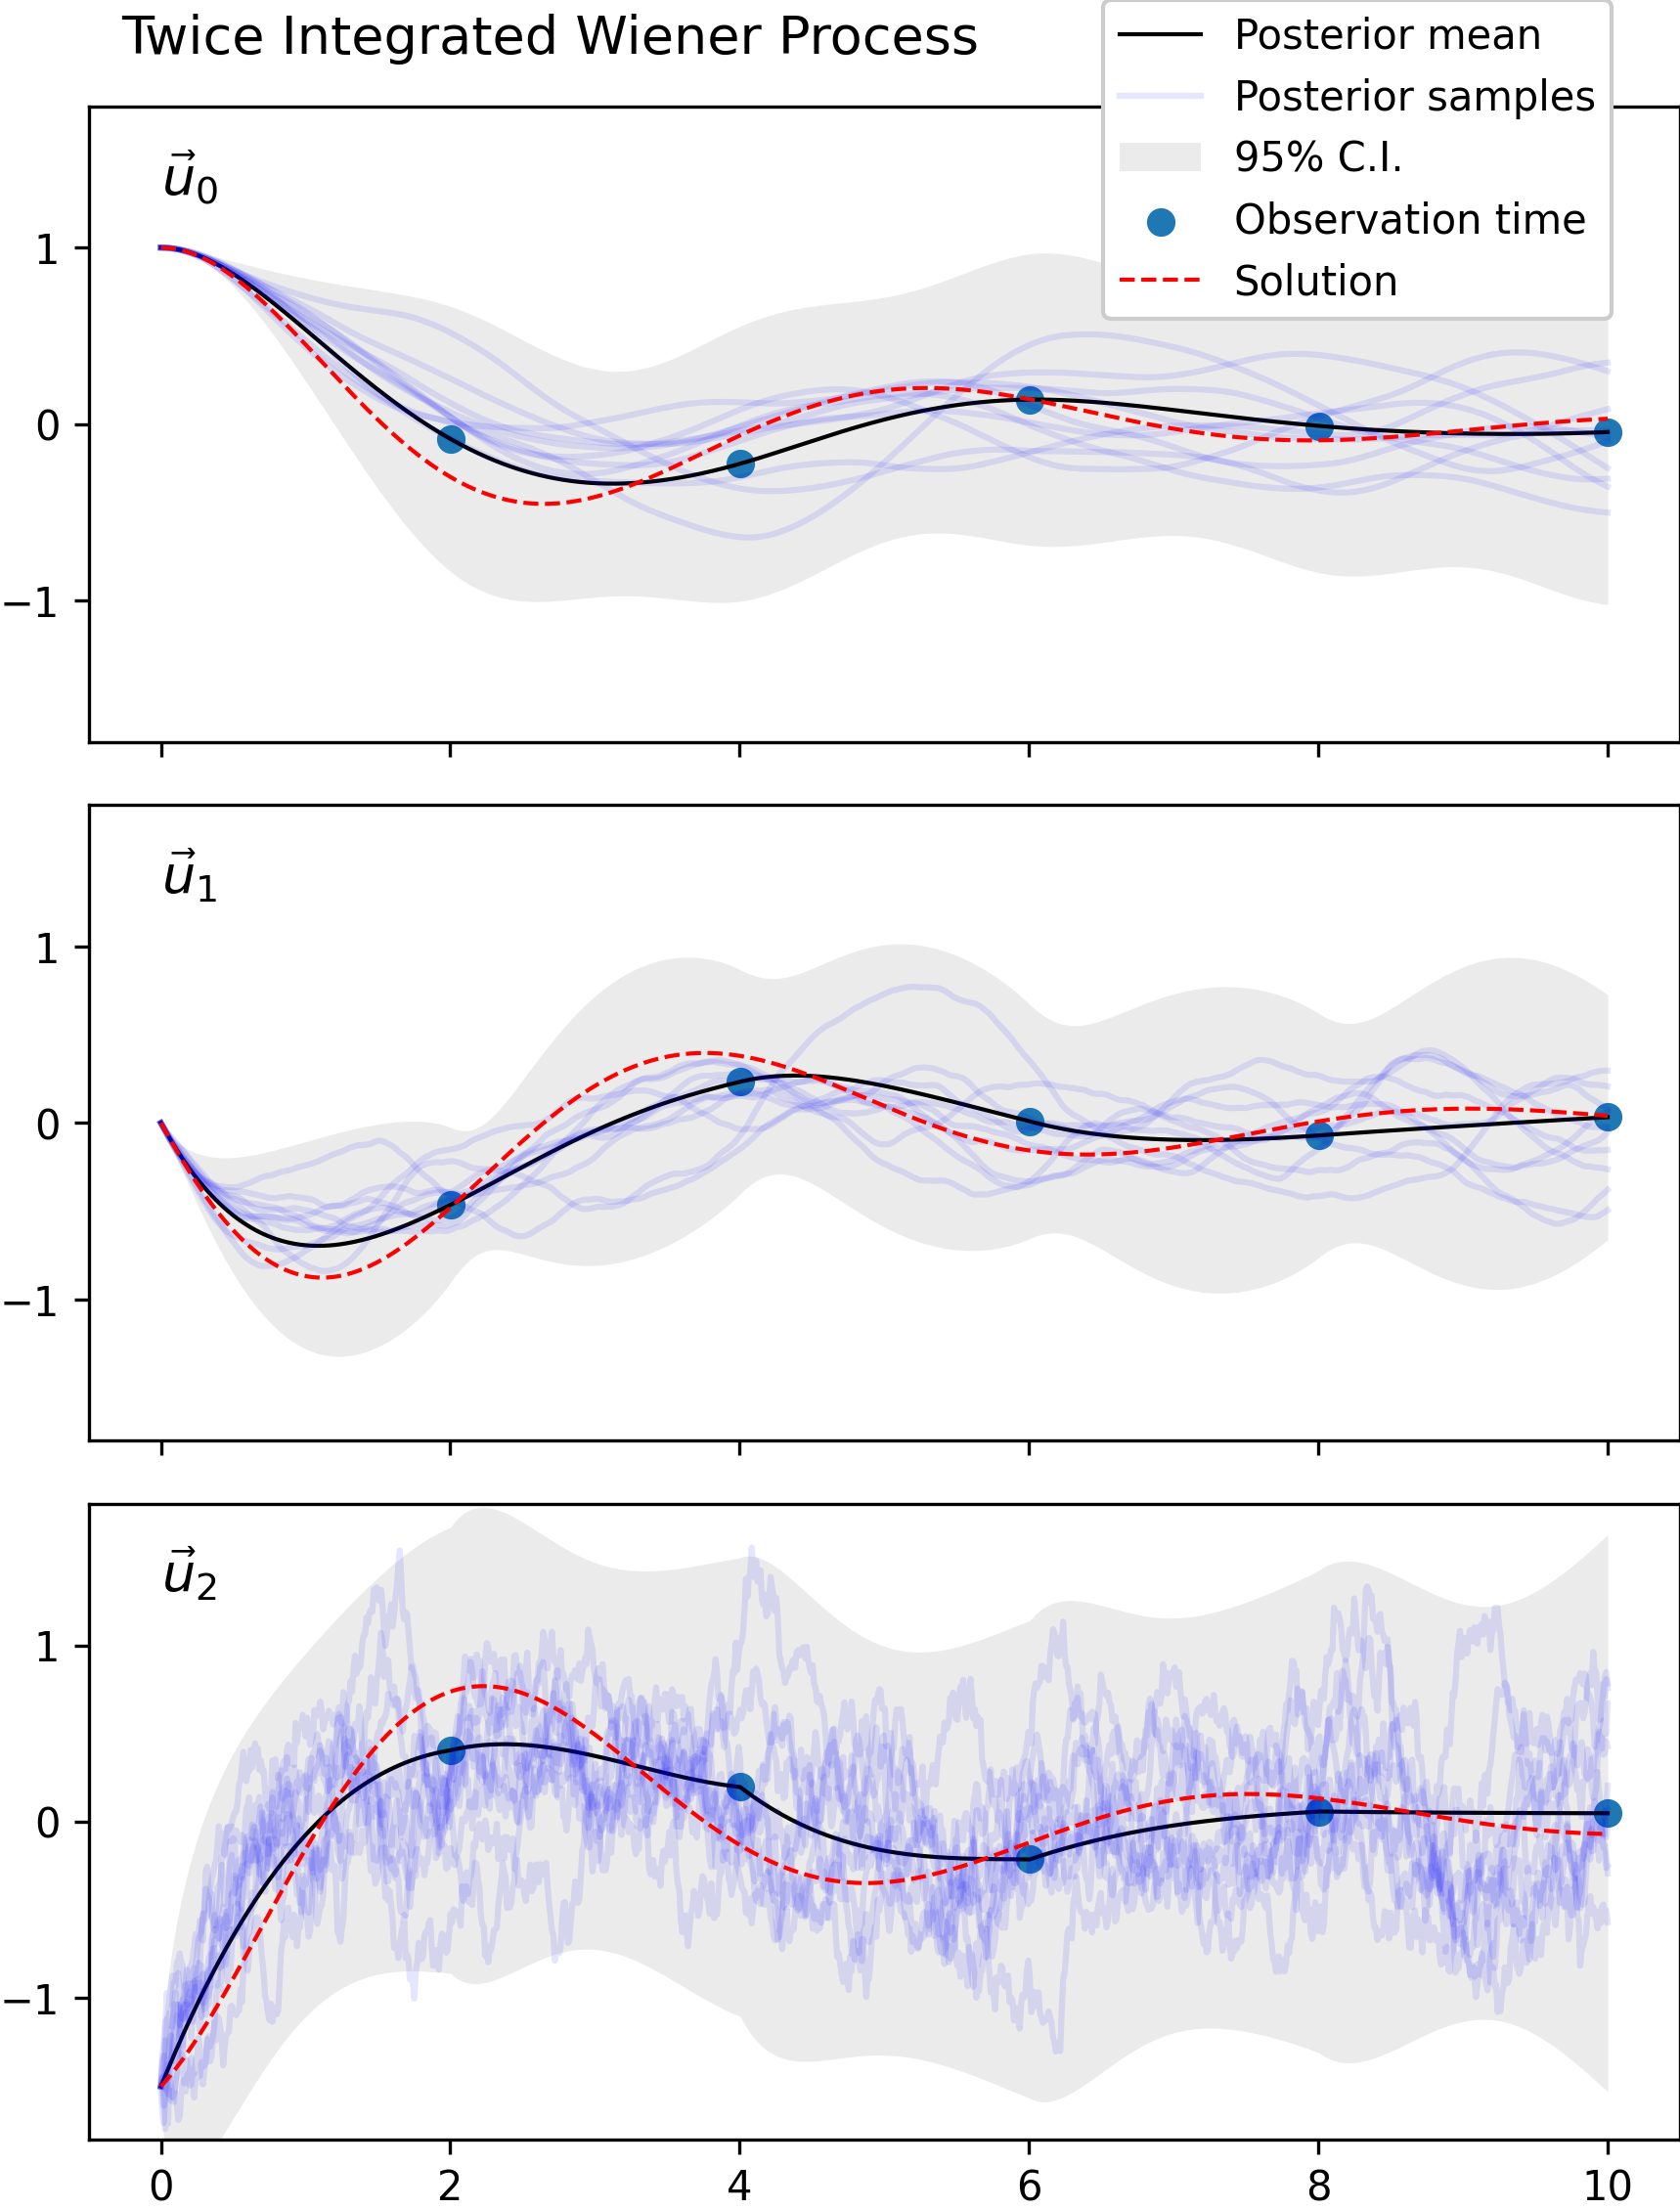
\includegraphics[width=\columnwidth]{../images/solving_damped_spring_small_state.png}       
        \captionof{figure}{Probabilistic numerical solution of the damped harmonic oscillator ODE. We are using a 2-times integrated Wiener process as prior. Note the increasing irregularity of the state components as we inspect higher derivates which have been integrated less frequently. The highest derivative here, $\vec{u}_2$, is no longer differentiable.}
    \end{center}
    \begin{center}
        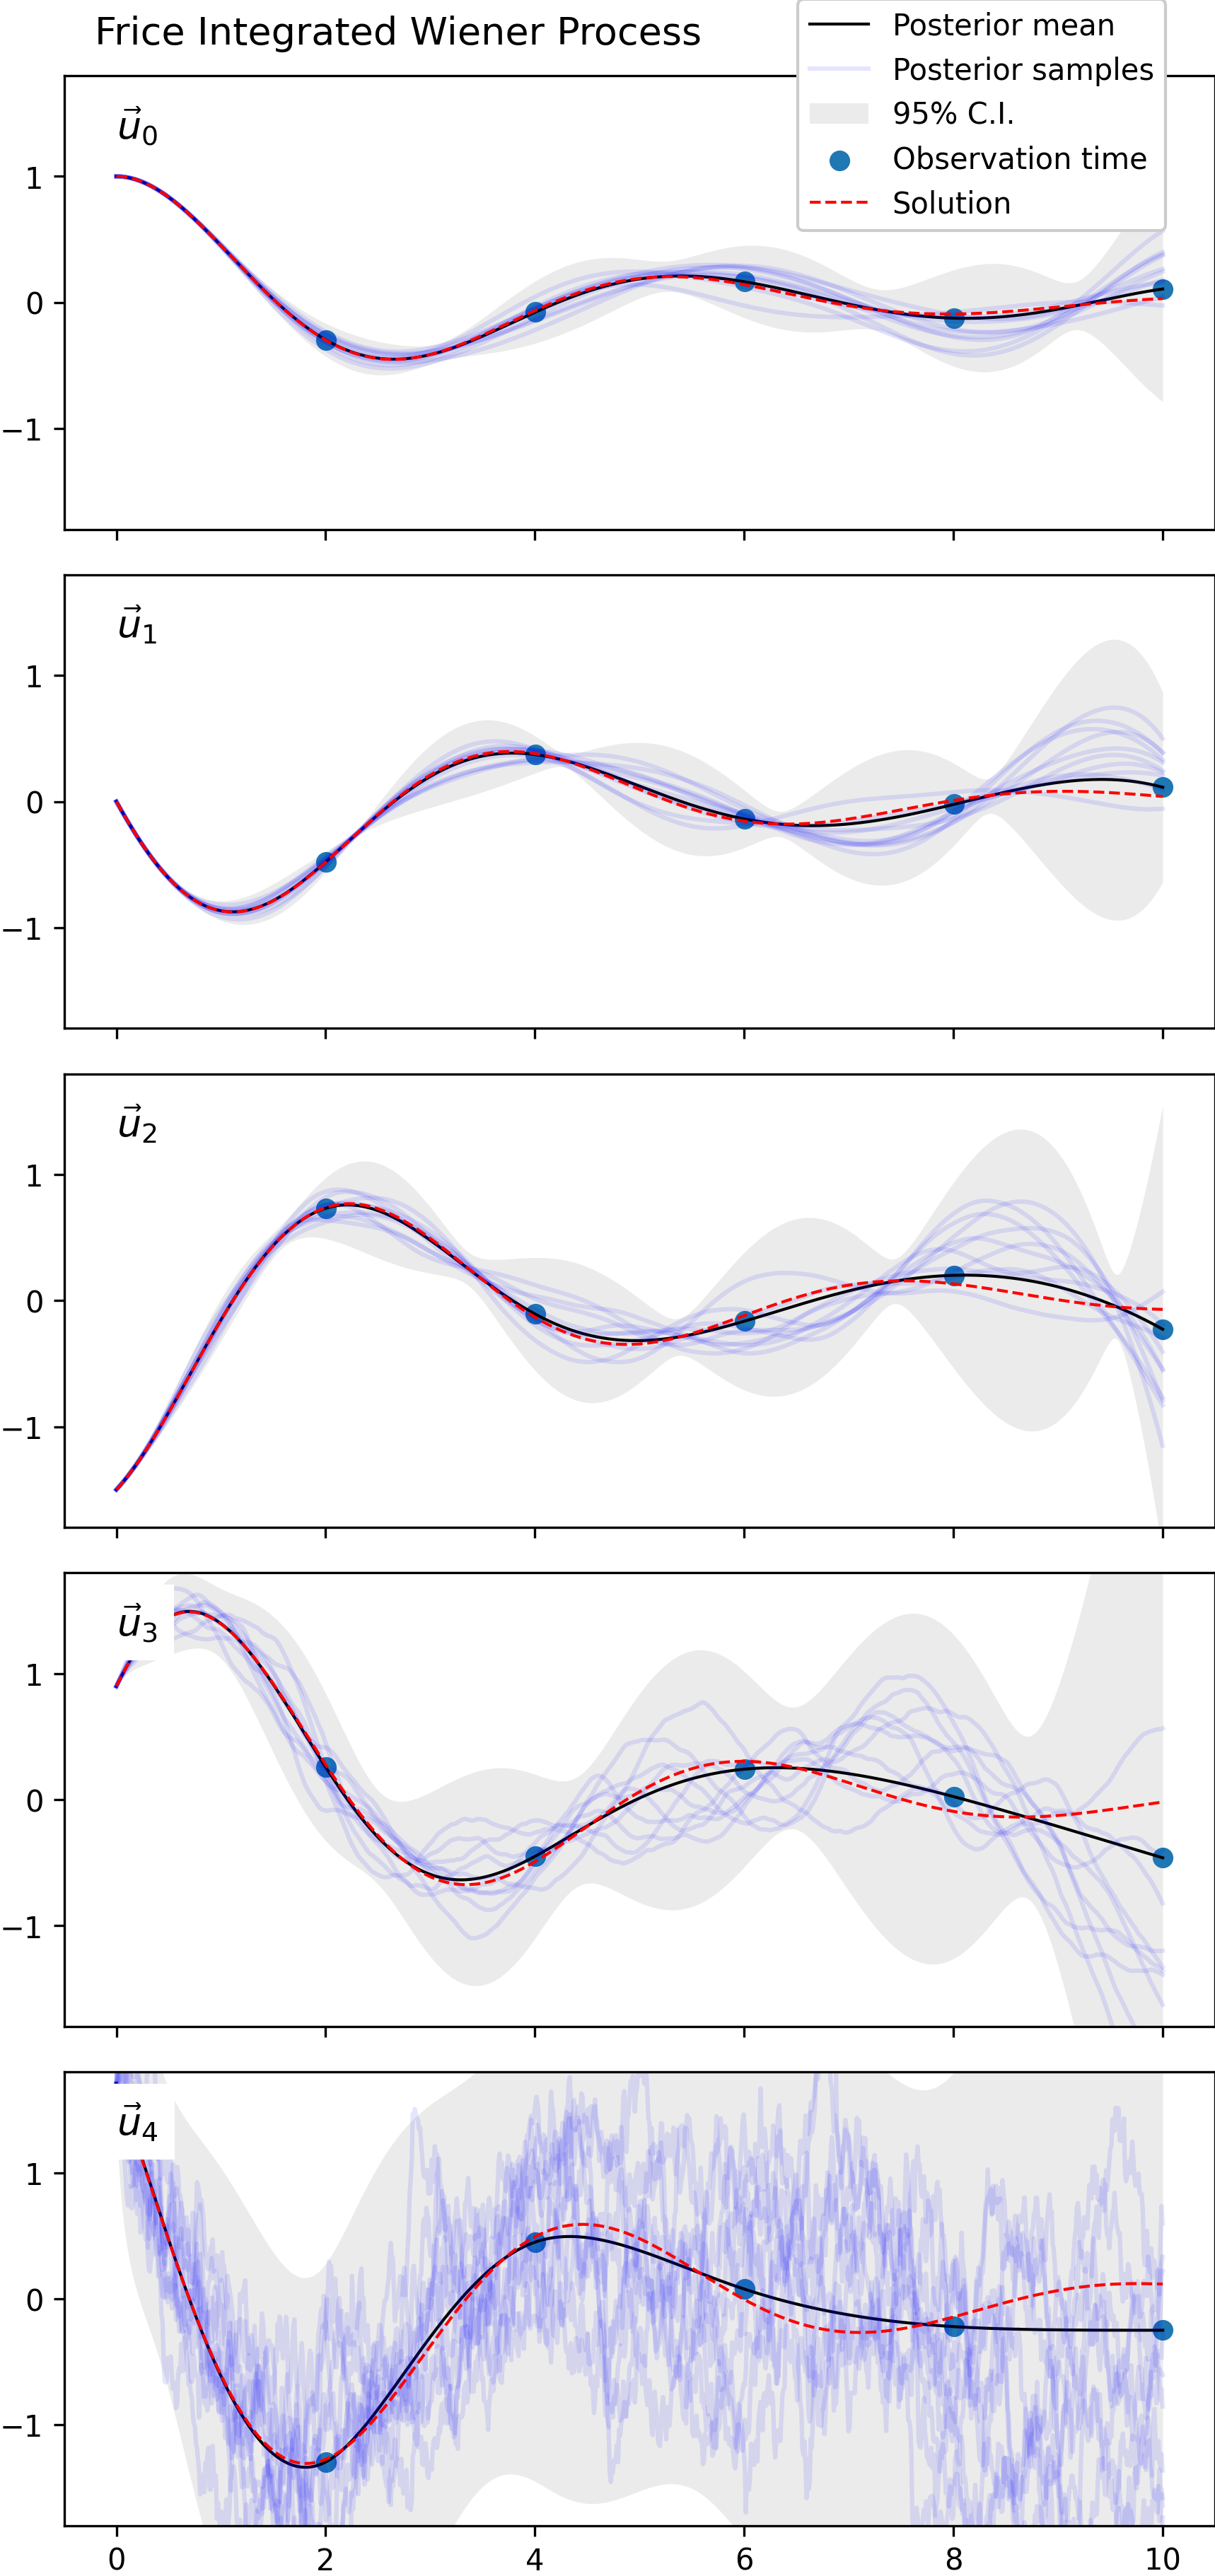
\includegraphics[width=\columnwidth]{../images/solving_damped_spring_big_state.png}
        \captionof{figure}{The same type of figure as above, but we are using a 4-times integrated Wiener process as the prior. We have conditioned on the same observations as in the previous figure, but there is much less uncertainty about the solution $\vec{u}_0$.}  
    \end{center}
}

\ifdefined\COMPILINGFROMMAIN
\else    
    \end{document}
\fi